\documentclass[cn,blue,12pt]{elegantbook}
\input{d:/tex/preamble}

\excludecomment{note}
\excludecomment{solution}
\renewcommand \tkt[1]{{\CJKunderline[hidden=true, skip=true, thickness=1pt]{#1}}}

\begin{document}

\maketitle

\tableofcontents

\mainmatter

\chapter{整式乘除法}%
\label{cha:整式乘除法}

\section{同底数幂的乘法}%
\label{sec:同底数幂的乘法}

\subsubsection{知识要点}%
\label{ssub:知识要点}

\begin{enumerate}
    \item 运算规则:同底数幂相乘,底数不变,指数相加.
    \item 公式:
        \begin{equation}
            a^m \cdot a^n = \tkt{a^{m+n}}(m,n\text{都是正整数)}
        \end{equation}
    \item 公式推导:\\
        \begin{align}
            a^m \cdot a^n & = \underbrace{(a\cdot a\cdot \cdots \cdot a)}_{m\text{个}a} \cdot \underbrace{(a\cdot a\cdot \cdots \cdot a)}_{n\text{个}a} \notag \\
                          & = \underbrace{a\cdot a\cdots a}_{(m+n)\text{个}} \notag \\
                          & = a^{m+n} \notag
        \end{align}
    \item 拓展公式:
        \begin{equation}
            a^m \cdot a^n \cdot a^p = \tkt{a^{m+n+p}}
        \end{equation}
\end{enumerate}

\subsubsection{例题}%
\label{ssub:例题}

\begin{liti}[resume]
\item 计算:
    \begin{liti}[resume]
    \item \(10^2 \times 10^3 = \)\tkt{\(10^5\)}
    \item \(10^5 \times 10^8 = \)\tkt{\(10^{13}\)}
    \item \(10^m \times 10^n = \)\tkt{\(10^{m+n}\)}
    \end{liti}
\item 计算:
    \begin{liti}
    \item \(2^m \times 2^n = \)\tkt{\(2^{m+n}\)}
    \item \((\frac{1}{7})^m \times (\frac{1}{7})^n = \)\tkt{\((\frac{1}{7})^{m+n}\)}
    \item \((-3)^m \times (-3)^n = \)\tkt{\((-3)^{m+n}\)}
    \end{liti}
\item 计算:
    \begin{liti}
    \item \((-3)^7 \times (-3)^6 = \)\tkt{\((-3)^{13}\)}
    \item \((\frac{1}{111})^3 \times \frac{1}{111} = \)\tkt{\((\frac{1}{111})^4\)}
    \item \(-x^3\cdot x^5 = \)\tkt{\(-x^8\)}
    \item \(b^{2m}\cdot b^{2m+1} = \)\tkt{\(b^{4m+1}\)}
    \end{liti}
\item 光在真空中的速度约为\(3\times 10^8 m/s\),太阳光照射到地球上大约需要 \(5\times 10^2 s\),地球距离太阳大约有多远.
\begin{solution}
        光在真空中的速度约为\(3\times 10^8 m/s\),太阳光照射到地球上大约需要 \(5\times 10^2 s\),地球距离太阳大约有多远.\\
\end{solution}
\end{liti}

\subsubsection{习题}%
\label{ssub:习题}
\paragraph{基础题}%
\label{par:基础题}

\begin{xiti}[resume]
\item 计算:
    \begin{xiti}[resume]
    \item \(5^2 \times 5^7=\)\tkt{\(5^9\)}
    \item \(7\times 7^3 \times 7^2= \) \tkt{\(7^6\)}
    \item -\(x^2 \cdot x^3 = \)\tkt{\(-x^5\)}
    \item \((-c)^3 \cdot (-c)^m = \)\tkt{\((-c)^{3+m}\)}
    \end{xiti}

\item 一种电子计算机每秒可做 \(4\times 10^9\)次运算,它工作 \(5\times 10^2s\)可做多少次运算?
\begin{solution}
        答:\(2\times 10^{12}\)\\
\end{solution}

\item 光在真空中的速度约为\(3\times 10^8 m/s\),太阳系以外距离地球最近的恒星是比邻星,它发出的光到达地球大约需要4.22年.一年以\(3\times 10^7s\)计算,比邻星与地球的距离约为多少?\\
\begin{solution}
        答:\(3\times 10^8 \times 3 \times 10^7 \times 4.22=3.798 \times 10^{16}m\)\\
\end{solution}
\item 计算:
    \begin{xiti}
    \item \(c\cdot c^{11}=\)\tkt{\(c^{12}\)}
    \item \(10^4 \times 10^2 \times 10=\)\tkt{\(10^7\)}
    \item \((-b)^3\cdot (-b)^2 = \)\tkt{\(-b^5\)}
    \item \(-b^3\cdot b^2 = \)\tkt{\(-b^5\)}
    \item \(x^{m-1}\cdot x^{m+1}(m>1) = \tkt{x^{2m}}\)
    \item \(a\cdot a^3 \cdot a^n = \)\tkt{\(a^{4+n}\)}
    \end{xiti}
\item 已知\(a^m=2,a^n=8,\text{求} a^{m+n} = \)\tkt{\(16\)}
\item 下列计算是否正确?如有错误请改正.
    \begin{xiti}
    \item \(a^3 \cdot a^2=a^6\)
\begin{solution}
            错. \(=a^5\)\\
\end{solution}
    \item \(b^4\cdot b^4=2b^4\)
\begin{solution}
            错. \(=b^8\)
\end{solution}
    \item \(x^5+x^5=x^{10}\)
\begin{solution}
            错.\(=2x^5\)\\
\end{solution}
    \item \(y^7\cdot y=y^8\)
\begin{solution}
            答:对\\
\end{solution}
    \end{xiti}
\item 在我国,平均每平方千米的土地一年从太阳得到的能量,相当于燃烧\(1.3\times 10^8 kg\)煤炭所产生的能量.我国\(960\text{万}km^2\)的土地上,一年从太阳得到的能量相当于燃烧多少千克的煤所产生的能量?
\begin{solution}
        答:\(1.3 \times 10^8 \times 960 \times 10^4 = 1.248 \times 10^{15} kg\)
\end{solution}
\item 某种细菌每过一分钟由1个分裂成成2个.\\
    (1)经过5min,1个细菌分裂成多少个?\\
    (2)这些细菌再继续分裂, \(t\)min后共分裂成多少个?
\begin{solution}
        答:(1) \(2^5\) 个\\
        (2) \(2^{5+t}\)个
\end{solution}
\end{xiti}

\section{幂的乘方与积的乘方}%
\label{sec:幂的乘方与积的乘方}

\subsubsection{知识要点}%
\label{ssub:知识要点}
\begin{enumerate}
    \item 幂的乘方
        \begin{enumerate}
            \item 运算规则:同底数幂的乘方,底数不变,指数相乘.
            \item 公式:
                \begin{equation}
                    (a^m)^n = \tkt{a^{mn}}(m,n\text{都是正整数)}
                \end{equation}
            \item 公式推导:\\
                \begin{align}
                    (a^m)^n & = \overbrace{(a^m\cdot a^m \cdots  a^m)}^{n\text{个}m} \notag\\
                            & = \overbrace{a^{m+m+\cdots +m}} \notag \\
                            & = a^{mn} \notag
                \end{align}
        \end{enumerate}
    \item 积的乘方
        \begin{enumerate}
            \item 运算规则:积的乘方等于\tkt{乘方的积}.
            \item 公式:
                \begin{equation}
                    (ab)^n = \tkt{a^nb^n}(n\text{是正整数)}
                \end{equation}
            \item 公式推导:\\
                \begin{align}
                    (ab)^n & = \underbrace{((ab)\cdot (ab) \cdots (ab))}_{n\text{个}ab} \notag\\
                           & = \underbrace{a\cdot a\cdots a}_{n\text{个}a} \cdot \underbrace{b\cdot b\cdots b}_{n\text{个}b}  \notag \\
                           & = a^nb^n \notag
                \end{align}
        \end{enumerate}

\end{enumerate}
\subsubsection{例题}%
\label{ssub:例题}

\paragraph{幂的乘方}%
\label{par:幂的乘方}

\begin{liti}[resume]
\item 计算:
    \begin{liti}
    \item \((6^2)^4\)=\tkt{\(6^8\)}
    \item \((a^2)^3\)=\tkt{\(a^6\)}
    \item \((a^m)^2\)=\tkt{\(a^{2m}\)}
    \item \((a^m)^n\)=\tkt{\(a^{mn}\)}
    \end{liti}
\item 计算:
    \begin{liti}
    \item \((10^2)^3=\)\tkt{\(10^6\)}
    \item \((b^5)^5=\)\tkt{\(b^{25}\)}
    \item \((a^n)^3=\)\tkt{\(a^{3n}\)}
    \item \(-(x^2)^m=\)\tkt{\(-x^{2m}\)}
    \item \((y^2)^3 \cdot y=\)\tkt{\(y^7\)}
    \item \(2(a^2)^6 - (a^3)^4 =\)\tkt{\(a^{12}\)}
    \end{liti}
\item 地球,木星,太阳可以近似地看作是球体.木星,太阳的半径分别约是地球的10倍和\(10^2\)倍,它们的体积分别约是地球的多少倍?(球体体积公式为\(V=\frac{4}{3}\pi r^3\),其中\(V\)是球的体积, \(r\)是球的半径.
\begin{solution}
        答:1000倍,1百万倍.\\
\end{solution}
\end{liti}

\paragraph{积的乘方}%
\label{par:积的乘方}

\begin{liti}[resume]
\item 计算:
    \begin{liti}
    \item \((3\times 5)^4=3^{(\tkt{\qquad})}\cdot 5^{(\tkt{\qquad})}\)
    \item \((3\times 5)^m=3^{(\tkt{\qquad})}\cdot 5^{(\tkt{\qquad})}\)
    \item \((ab)^n=a^{(\tkt{\qquad})}\cdot b^{(\tkt{\qquad})}\)
    \end{liti}
\item 计算:
    \begin{liti}[resume]
    \item \((3x)^2=\)\tkt{\(9x^2\)}
    \item \((-2b)^5=\)\tkt{\(-32b^5\)}
    \item \((-2xy)^4=\)\tkt{\(16x^4y^4\)}
    \item \((3a^2)^n=\)\tkt{\(3^na^{2n}\)}
    \end{liti}
\item 地球可以近似地看作是球体,地球的半径约为\(6\times 10^3 km\),它的体积大约是多少立方千米?(\(\pi\)取近似值3.14)
\begin{solution}
        答:\(V=\frac{4}{3}\pi r^3 = \frac{4}{3}\pi\times (6\times 10^3)^3=9.04\times 10^{11}m^3\)\\
\end{solution}
\end{liti}

\subsubsection{习题}%
\label{ssub:习题}

\paragraph{幂的乘方}%
\label{par:幂的乘方}

\begin{xiti}[resume]
\item 计算:
    \begin{xiti}
    \item \((10^3)^3=\)\tkt{\(10^9\)}
    \item \(-(a^2)^5=\)\tkt{\(-a^{10}\)}
    \item \((x^3)^4\cdot x^2=\)\tkt{\(x^{14}\)}
    \end{xiti}
\item 计算:
    \begin{xiti}
    \item \([(\frac{1}{3})^3]^2=\)\tkt{\((\frac{1}{3})^6\)}
    \item \((a^4)^2=\)\tkt{\(a^8\)}
    \item \(-(b^5)^2=\)\tkt{\(-b^{10}\)}
    \item \((y^2)^{2n}=\)\tkt{\(y^{4n}\)}
    \item \((b^n)^3=\)\tkt{\(b^{3n}\)}
    \item \((x^3)^{3n}=\)\tkt{\(x^{9n}\)}
    \end{xiti}
\item 计算:
    \begin{xiti}
    \item \(-p\cdot (-p)^4=\)\tkt{\(-p^5\)}
    \item \((a^2)^3\cdot (a^3)^2=\)\tkt{\(a^{12}\)}
    \item \((t^m)^2\cdot t=\)\tkt{\(t^{2m+1}\)}
    \item \((x^4)^6-(x^3)^8=\)\tkt{\(0\)}
    \end{xiti}
\item 下面的计算是否正确?如有错误请改正
    \begin{xiti}
    \item \((x^3)^3=x^6\)
\begin{solution}
            错.\(x^9\)\\
\end{solution}
    \item \(a^6\cdot a^4=a^{24}\)
\begin{solution}
            \(a^{10}\)\\
\end{solution}
    \end{xiti}
\item \(1m=10dm=100cm\),那么\(1m^2\)等于多少\(dm^2\)?等于多少\(cm^2\)?
\begin{solution}
        \(1m^2=100dm^2=10^4cm^2\)\\
\end{solution}
\item \(1m=10dm=100cm\),那么\(1m^3\)等于多少\(dm^3\)?等于多少\(cm^3\)?
\begin{solution}
        \(1m^3=1000dm^3=10^6cm^3\)\\
\end{solution}
\item \(1cm=10^{-1}dm=10^{-2}m\),那么\(1cm^2\)等于多少\(dm^2\)?等于多少\(m^2\)?
\begin{solution}
        \(1cm^2=10^{-2}dm^2=10^{-4}m^2\)\\
\end{solution}
\item \(1cm=10^{-1}dm=10^{-2}m\),那么\(1cm^3\)等于多少\(dm^3\)?等于多少\(m^3\)?
\begin{solution}
        \(1cm^3=10^{-3}dm^3=10^{-6}m^3\)\\
\end{solution}
\end{xiti}

\paragraph{积的乘方}%
\label{par:积的乘方}

\begin{xiti}[resume]
\item 计算:
    \begin{xiti}
    \item (\(3b)^2=\)\tkt{\(9b^2\)}
    \item \(-(ab)^2=\)\tkt{\(-a^2b^2\)}
    \item \(-a^3+(-4a)^2a=\)\tkt{\(-15a^3\)}
    \item \((y^2z^3)^3=\)\tkt{\(y^6z^9\)}
    \end{xiti}
\item 计算:
    \begin{xiti}
    \item (\(-3n)^3=\)\tkt{\(-27n^3\)}
    \item \((5xy)^3=\)\tkt{\(125x^3y^3\)}
    \item \(-a^3+(-4a)^2a=\)\tkt{\(15a^3\)}
    \end{xiti}
\item 计算:
    \begin{xiti}
    \item \((xy^4)^m=\)\tkt{\(x^my^{4m}\)}
    \item \(-(p^2q)^n=\)\tkt{\(-p^{2n}q^n\)}
    \item \((xy^{3n})^2+(xy^6)^n=\)\tkt{\(x^2y^{6n}+x^ny^{6n}\)}
    \item \((-3x^3)^2-[(2x)^2]^3=\)\tkt{\(-55x^6\)}
    \end{xiti}
\item 下面的计算是否正确?如有错误请改正.
    \begin{xiti}
    \item \((ab^4)^4=ab^8\)
\begin{solution}
            错.\(a^4b^{16}\)\\
\end{solution}
    \item \((-3pq)^2=-6p^2q^2\)
\begin{solution}
            错.\(9p^2q^2\)\\
\end{solution}
    \end{xiti}
\item 简便运算:
    \begin{xiti}
    \item \(2^2 \times 3\times 5^2\)
\begin{solution}
            \(=2^2\times 5^2\times 3 = (2\times 5)^2\times 3=300\)\\
\end{solution}
    \item \(2^4 \times 3^2\times 5^3\)
\begin{solution}
            \(=(2\times 5)^3 \times 2 \times 3^2 = 1000\times 2 \times 9=18000\)\\
\end{solution}
    \end{xiti}
\item \((abc)^n=\)\tkt{\(a^nb^nc^n\)}
\end{xiti}

\section{同底数幂的除法}%
\label{sec:同底数幂的除法}

\subsubsection{知识要点}%
\label{ssub:知识要点}
\begin{enumerate}
    \item 同底数幂的除法
        \begin{enumerate}
            \item 运算规则:同底数幂相除,底数不变,指数相减.
            \item 公式:
                \begin{eqnarray}
                    a^m \div  a^n = \tkt{a^{m-n}}\\
                    a^0=1(a\ne 0)\\
                    a^{-p}=\frac{1}{a^p}(a\ne 0)
                \end{eqnarray}
            \item 公式推导:\\
                \begin{align}
                    a^m \div  a^n & = \frac{\overbrace{a\cdot a\cdots a}^{m\text{个}a}}{\underbrace{a\cdot a\cdots a}_{n\text{个}a}}\notag \\
                                  & = \overbrace{a\cdot a\cdots a}^{(m-n)\text{个}} \notag \\
                                  & = a^{m-n} \notag
                \end{align}
        \end{enumerate}
    \item 科学记数法
        \begin{enumerate}
            \item 定义:把一个数表示成\(a\)与\(10\)的\(n\)次幂相乘的形式\((1\le |a|<10,n\)为整数),当数的绝对值小于1时,n是负整数.用科学记数法可以很方便的表示一些绝对值较大或较小的数.
            \item 科学记数法的精确度:\(a \times 10^n\)的的精确度以\(a\)的最后一个数在原数中的数位为准. 如13600精确到十位记作\(1.360 \times 10^4\);精确到百位记作\(1.36 \times 10^4\);精确到千位记作\(1.3\times 10^5\).
        \end{enumerate}
\end{enumerate}
\subsubsection{例题}%
\label{ssub:例题}

\paragraph{同底数幂的除法}%
\label{par:同底数幂的除法}

\begin{liti}[resume]
\item 计算:
    \begin{liti}
    \item \(10^{12} \div 10^9\) = \tkt{\(10^3\)}
    \item \(10^{m} \div 10^n\) = \tkt{\(10^{m-n}\)}
    \item \((-3)^{m} \div (-3)^n\) = \((-3)^{m-n}\)
    \end{liti}
\item 计算:
    \begin{liti}
    \item \(a^7 \div a^4\) = \tkt{\(a^3\)}
    \item \((-x)^6 \div (-x)^3\) = \tkt{\(-x^3\)}
    \item \((xy)^4 \div (xy)\) = \tkt{\(x^3y^3\)}
    \item \(b^{2m+2} \div (b^2)\) = \tkt{\(b^{2m}\)}
    \end{liti}
\item 计算:
    \begin{liti}
        \begin{multicols}{2}
        \item \(10^4=10 000\)
        \item \(10^{(\tkt{\qquad})}=1 000\)
        \item \(10^{(\tkt{\qquad})}=1 00\)
        \item \(10^{(\tkt{\qquad})}=1 0\)
        \item \(2^4=16\)
        \item \(2^{(\tkt{\qquad})}=8\)
        \item \(2^{(\tkt{\qquad})}=4\)
        \item \(2^{(\tkt{\qquad})}=2\)
        \end{multicols}
    \end{liti}
\item 用小数或分数表示下列各数:
    \begin{liti}
    \item \(10^{-3}=\)\tkt{\(0.001\)}
    \item \(7^0\times 8^{-2}=\)\tkt{\(\frac{1}{64}\)}
    \item \(1.6 \times 10^{-4}= \) \tkt{\(0.00016\)}
    \end{liti}
\item 计算:
    \begin{liti}[resume]
    \item \(7^{-3} \div 7^{-5}=\)\tkt{49}
    \item \(3^{-1} \div 3^6=\)\tkt{\(3^{-7}\)}
    \item \((\frac{1}{2})^{-5} \div (\frac{1}{2})^2=\)\tkt{\(2^7\)}
    \item \((-8)^{0} \div (-8)^{-2}=\)\tkt{\(64\)}
    \end{liti}
\item 一种液体每升含有\(10^{12}\)个有害细菌,为了试验某种杀菌剂的效果,科学家们进行了实验,发现1滴杀菌剂可以杀死\(10^9\)个此种细菌.要将\(1L\)液体中的有害细菌全部杀死,需要这种杀菌剂多少滴?
\begin{solution}
        \(\frac{10^{12}}{10^9}=10^3\)滴\\
\end{solution}
\end{liti}

\paragraph{科学记数法}%
\label{par:科学记数法}

\begin{liti}[resume]
\item 用科学记数法表示:
    \begin{liti}[resume]
    \item 细胞的直径只有1微米\((\mu m)\),即\(0.000,001m\)
\begin{solution}
            \(1\times 10^{-6}\)\metre \\
\end{solution}
    \item 某种计算机完成一次基本运算的时间约为1纳秒\((ns)\),即\(0.000,000,001s\)
\begin{solution}
            \(1\times 10^{-9}\)\second \\
\end{solution}
    \item 一个氧原子的质量为\(0.000,000,000,000,000,000,000,026,57kg\)
\begin{solution}
            \(2.657 \times 10^{-26}\) \kilogram \\
\end{solution}
    \end{liti}
\item 用科学记数法表示:
    \begin{liti}[resume]
    \item 0.000,000,000,1 = \tkt{\(1\times 10^{-10}\)}
    \item 0.000,000,000,002,9 = \tkt{\(2.9 \times 10^{-12}\)}
    \item 0.000,000,001,295 = \tkt{\(1.295 \times 10^{-9}\)}
    \end{liti}
\item PM2.5是指大气中直径小于或等于\(2.5 \mu m\)的颗粒物,也称为可入肺颗粒物.假设一种可入肺颗粒物的直径约为2.5\(\mu m\),相当于多少米?多少个这样的颗粒物首尾相接连起来能达到1m?
\begin{solution}
        \(2.5\times 10^{-6} \metre; \frac{1}{2.5\times 10^{-6}}= 4\times 10^5 = 400000 \)个\\
\end{solution}
\end{liti}

\subsubsection{习题}%
\label{ssub:习题}

\paragraph{同底数幂的除法}%
\label{par:同底数幂的除法}

\begin{xiti}[resume]
\item 计算:
    \begin{xiti}
    \item \(x^{12}\div x^4=\)\tkt{\(x^8\)}
    \item \((-y)^3 \div (-y)^2=\)\tkt{\(-y\)}
    \item \(-(k^6 \div k^6)=\)\tkt{\(-1\)}
    \item \((-r)^5 \div r^4=\)\tkt{\(-r\)}
    \item \(m \div m^0=\)\tkt{\(m\)}
    \item \((mn)^5 \div (mn)=\)\tkt{\(m^4n^4\)}
    \end{xiti}
\item 计算:
    \begin{xiti}
    \item \(2^{13}\div 2^7\)=\tkt{\(2^6\)}
    \item \((-\frac{3}{2})^6 \div (-\frac{3}{2})^2\)=\tkt{\(\frac{81}{16}\)}
    \item \(a^{11} \div a^5\)=\tkt{\(a^6\)}
    \item \((-x)^7 \div (-x)\)=\tkt{\(x^6\)}
    \item \(a^{-4} \div a^{-6}\)=\tkt{\(a^2\)}
    \item \(6^{2m+1} \div 6^m\)=\tkt{\(6^{m+1}\)}
    \item \(5^{n+1} \div 5^{3n+1}\)=\tkt{\(5^{-2n}\)}
    \item \(9^n \div 9^{n+2}\)=\tkt{\(\frac{1}{81}\)}
    \end{xiti}
\item 用小数或分数表示下列各数:
    \begin{xiti}
    \item \((\frac{1}{2})^0\)= \tkt{\(1\)}
    \item \(3^{-3}\)= \tkt{\(\frac{1}{27}\)}
    \item \(1.3 \times 10^{-5}\)= \tkt{\(0.000013\)}
    \item \(5^{-2}\)= \tkt{\(\frac{1}{25}\)}
    \end{xiti}
\item 下面的计算是否正确?如有错误请改正
    \begin{xiti}
    \item \(a^6 \div a = a^6\)\tkt{错.\(a^5\)}
    \item \(b^6 \div b^3 = b^2\)\tkt{错.\(b^2\)}
    \item \(a^{10} \div a^9 = a\)\tkt{对.}
    \item \((-bc)^4 \div (-bc)^2 = -b^2c^2\)\tkt{错.\(b^2c^2\)}
    \end{xiti}
\item 某种细胞分裂时,1个细胞分裂1次变为2个,分裂2次变为4个,分裂3次变为8个, \(\cdots\cdots\)你能由此说明\(2^0=1\)的合理性吗?
\begin{solution}
        不分裂,即分裂次数为0时,结果为1.\\
\end{solution}
\end{xiti}

\paragraph{科学记数法}%
\label{par:科学记数法}

\begin{xiti}[resume]
\item 用科学计数法表示:
    \begin{xiti}
    \item 0.000,000,72= \tkt{\(7.2\times 10^{-7}\)}
    \item 0.000,861= \tkt{\(8.52\times 10^{-4}\)}
    \item 0.000,000,000,342,5= \tkt{\(3.425 \times 10^{-10}\)}
    \end{xiti}
\item 1个电子的质量为\(0.000,000,000,000,000,000,000,000,000,911g\),用科学记数法表示这个数.
\begin{solution}
        \(9.11 \times 10^{-28} \gram \)\\
\end{solution}
\item 纳米\((nm)\)是一种长度单位, \(1nm\)为十亿分之一米,直径为\(1nm\)的球与乒乓球相比,相当于乒乓球与地球相比.用科学记数法表示纳米与米的单位转换.
\begin{solution}
        \(1\nano\meter = 10^{-9} \metre \)
\end{solution}
\item 用科学记数法表示万,亿.
\begin{solution}
        \(1\times 10^4, 1\times 10^8\)
\end{solution}
\item 国际单位制词头用来表示单位的倍数和分数,常用的词头有:兆千(个)毫微纳,其中前面一个为后面一个的1000倍,写出它们的一般形式,然后用科学记数法表示.
\begin{solution}
        兆:百万,毫:千分之一,微:百万分之一,纳:十亿分之一.\\
        \(M:10^6, K:10^3, 10^0, m:10^{-3}, \mu :10^{-6}, \nano :10^{-9}\)
\end{solution}
\item 用科学记数法表示:
    \begin{xiti}
    \item 0.007,398= \tkt{\(7.398 \times 10^{-3}\)}
    \item 0.000,022,6= \tkt{\(2.26 \times 10^{-5}\)}
    \item 0.000,000,000,054,2= \tkt{\(5.42 \times 10^{-11}\)}
    \item 0.000,000,000,000,000,000,000,199,4= \tkt{\(1.994 \times 10^{-22}\)}
    \end{xiti}
\item 空气的密度是\(1.293 \times 10^{-3}g/cm^3\),用小数把它表示出来.
\begin{solution}
        \(0.001293\) \gram\per\cubic{\centi\metre}\\
\end{solution}
\item 一个铁原子的质量为\(0.000,000,000,000,000,000,000,000,092,88kg\),用科学记数法表示.
\begin{solution}
        \(9.288 \times 10^{-26} \kilogram \)\\
\end{solution}
\item 人体内一种细胞的直径约为\(1.56 \mu m\),相当于多少米?多少个这样的细胞首尾连接起来能达到\(1m\)?
\begin{solution}
        \(1.56 \milli\metre = 1.56 \times 10^{-6} \metre = 0.000,001,56 \metre \)\\
        \(\frac{1}{1.56 \times  10^{-6}}= 6.41 \times 10^5 = 641,000\)个
\end{solution}
\end{xiti}

\section{整式的乘法}%
\label{sec:整式的乘法}

\subsubsection{知识要点}%
\label{ssub:知识要点}
\begin{enumerate}
    \item 单项式与单项式相乘:把系数,相同字母的幂分别相乘,其余字母连同它的指数不变作为积的因式.
    \item 单项式与多项式相乘:根据分配率用单项式去乘多项式的每一项,再把所得的积相加.
    \item 多项式与多项式相乘:先用一个多项式的每一项乘另一个多项式的每一项,再把所得的积相加.
\end{enumerate}

\subsubsection{例题}%
\label{ssub:例题}
\paragraph{单项式与单项式相乘}%
\label{par:单项式与单项式相乘}
\begin{liti}[resume]
\item 计算:
    \begin{liti}
    \item \(3a^2b\cdot 2ab^3\)= \tkt{\(6a^3b^3\)}
    \item \(xyz\cdot y^2z\)= \tkt{\(xy^3z^2\)}
    \item \(2xy^2\cdot \frac{1}{3}xy\)= \tkt{\(\frac{2}{3}x^2y^3\)}
    \item \(-2a^2b^3\cdot (-3a)\)= \tkt{\(2a^4b^3\)}
    \item \(7xy^2z\cdot (2xyz)^2\)= \tkt{\(14x^3y^4z^3\)}
    \end{liti}
\item 计算:
    \begin{liti}[resume]
    \item \(5x^3 \cdot 2x^2y\) = \tkt{\(10x^5y\)}
    \item \(-3ab \cdot (-4b^2)\) = \tkt{\(12ab^3\)}
    \item \(3ab \cdot 2a\) = \tkt{\(6a^2b\)}
    \item \(yz \cdot 2y^2z^2\) = \tkt{\(2y^3z^3\)}
    \item \((2x^2y)^3\cdot (-4xy^2)\)  = \tkt{\(-32x^7y^5\)}
    \item \(\frac{1}{3}a^3b\cdot 6a^5b^2c\cdot (-ac^2)^2\)= \tkt{\(2a^{10}b^3c^5\)}
    \end{liti}
\item 如图,第一幅画的画面大小与纸的大小相同,第二幅画的画面在纸的上,下方各留有\(\frac{1}{8}x\, m\)的空白.\\
    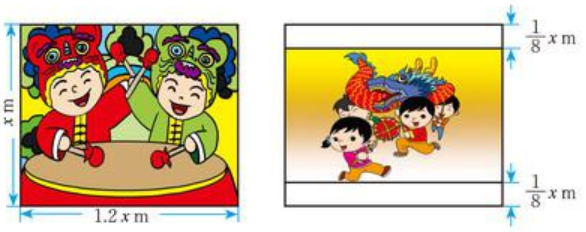
\includegraphics[width=0.5\linewidth]{pic/20200429001.png}\\
    (1)第一幅和第二幅画的画面面积分别是多少平方米?\\
    (2)若把图中的\(1.2x\)改为\(mx\),其他不变,则两幅画的面积又该怎样表示?
\begin{solution}
        (1) \(1.2x^2 \squaremetre ; 1.2x \cdot (1-2\times \frac{1}{8})x = 0.9 x^2 \squaremetre \)\\
        (2) \(mx^2 \squaremetre ; \frac{3}{4} mx^2 \squaremetre \)
\end{solution}
\end{liti}

\paragraph{单项式与多项式相乘}%
\label{par:单项式与多项式相乘}

\begin{liti}[resume]
\item 计算:
    \begin{liti}
    \item \(2ab(5ab^2+3a^2b)\)= \tkt{\(10a^2b^3+6a^3b^2\)}
    \item \((\frac{2}{3}ab^2-2ab)\cdot \frac{1}{2}ab\)= \tkt{\(\frac{1}{3}a^2b^3 - a^2b^2\)}
    \item \(5m^2n(2n+3m-n^2)\)= \tkt{\(10 m^2n^2 + 15m^3n - 5 m^2n^3\)}
    \item \(2(x+y^2z+xy^2z^3)\cdot xyz\)= \tkt{\(2x^2yz + 2xy^3z^2 + 2x^2y^3z^4\)}
    \end{liti}
\item 计算:
    \begin{liti}
    \item \(a(a^2m+n)\)= \tkt{\(a^3m+a_n\)}
    \item \(b^2(b+3a-a^2)\) = \tkt{\(b^3+3ab^2-a^2b\)}
    \item \(x^3y(\frac{1}{2}xy^3-1)\) = \tkt{\(\frac{1}{2}x^4y^4-x^3y\)}
    \item \(4(e+f^2d)\cdot ef^2d\) = \tkt{\(4e^2f^2d + 4ef^4d^2\)}
    \end{liti}
\end{liti}

\paragraph{多项式与多项式相乘}%

\begin{liti}[resume]
\item 计算:
    \begin{liti}
    \item \((1-x)(0.6-x)\) = \tkt{\(x^2 - 1.6x + 0.6\)}
    \item \((2x+y)(x-y)\) = \tkt{\(2x^2 - xy -y^2\)}
    \end{liti}
\item 计算:
    \begin{liti}
    \item \((m+2n)(m-2n)\) = \tkt{\(m^2-4n^2\)}
    \item \((2n+5)(n-3)\) = \tkt{\(2n^2 - n -15\)}
    \item \((x+2y)^2\) = \tkt{\(x^2+4xy+4y^2\)}
    \item \((ax+b)(cx+d)\) = \tkt{\(acx^2 + (ad+bc)x + bd\)}
    \end{liti}
\end{liti}
\subsubsection{习题}%
\label{ssub:习题}

\paragraph{单项式与单项式相乘}%
\begin{xiti}[resume]
\item 计算:
    \begin{xiti}
    \item \(4xy\cdot (-2xy^3)\) = \tkt{\(-8x^2y^4\)}
    \item \(a^3b \cdot ab^5c\) = \tkt{\(a^4b^6c\)}
    \item \(2x^2y \cdot (-xy)^2\) = \tkt{\(-2x^4y^3\)}
    \item \( \frac{2}{5}x^2y^3 \cdot \frac{5}{8}xyz\) = \tkt{\(\frac{1}{4}x^3y^4z\)}
    \item \(-xy^2z^3 \cdot (-x^2y)^3\) = \tkt{\(x^7y^5z^3\)}
    \item \(-ab^3 \cdot 2abc^2 \cdot (a^2c)^3\) = \tkt{\(-2a^7b^4c^5\)}
    \end{xiti}
\end{xiti}

\paragraph{单项式与多项式相乘}%
\label{par:单项式与多项式相乘}
\begin{xiti}[resume]
\item 计算:
    \begin{xiti}
    \item \(5x(2x^2-3x+4)\) = \tkt{\(10x^3-15x^2+20x\)}
    \item \(-6x(x-3y)\) = \tkt{\(-6x^2+18xy\)}
    \item \(-2a^2(\frac{1}{2}ab+b^2)\) = \tkt{\(-a^3b-2a^2b^2\)}
    \item \((\frac{2}{3}x^2y-6xy) \cdot \frac{1}{2}xy^2\) = \tkt{\(\frac{1}{3}x^3y^3-3x^2y^3\)}
    \end{xiti}
\item 分别计算下面图中阴影部分的面积.\\
    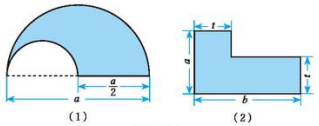
\includegraphics[width=0.5\linewidth]{pic/20200429002.png}\\
\begin{solution}
        (1) 阴影=\(\frac{1}{2}\)(大圆-小圆); 大圆半径=\(\frac{a}{2}\),小圆半径=\(\frac{a}{4}\)\\
        所以:阴影面积=\(\frac{1}{2}(\pi ( \frac{1}{2}a )^2-\pi (\frac{1}{4}a)^2)=\frac{3}{32}\pi a^2\)\\
        (2) 阴影=大长方形-空白小长方形; 大长方形边长为\(a, b\), 小长方形边长为 \(b-t,a-t\)\\
        所以:阴影面积\(=ab-(b-t)(a-t)=ab-ab+bt+at-t^2 = at+bt-t^2 \)
\end{solution}
\item 如图,按照图中棋子的摆法,第\(n\)个图形中共有多少枚棋子?\\
    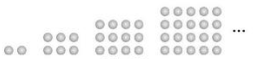
\includegraphics[width=0.5\linewidth]{pic/20200429003.png}\\
\begin{solution}
        规律:\(2\times 1, 3\times 2, 4\times 3, 5\times 4 \cdots\)\\
        所以,第\(n\)个图形: \((n+1)n=n^2+n\)
\end{solution}
\end{xiti}

%待完成习题
\paragraph{多项式与多项式相乘}%
\begin{xiti}[resume]
\item 计算:
    \begin{xiti}
    \item \((x+y)(a+2b)\) = \tkt{\(ax + ay + 2bx + 2by\)}
    \item \((2a+3)(\frac{3}{2}b+5)\) = \tkt{\(3ab+10a+\frac{9}{2}b+15\)}
    \item \((2x+3)(-x-1)\) = \tkt{\(-2x^2-5x-3\)}
    \item \((-2m-1)(3m-2)\) = \tkt{\(-6m^2+m+2\)}
    \item \((x-y)^2\) = \tkt{\(x^2-2xy+y^2\)}
    \item \((-2x+3)^2\) = \tkt{\(4x^2-12x+9\)}
    \end{xiti}
\item
    \begin{xiti}
    \item 观察:\(4\times 6=24, 14\times 16 =224, 24\times 26=624, 34\times 36=1224, \cdots\)\\
        发现其中的规律并用代数式表示.
    \item 利用(1)中的规律计算\(124\times 126.\)
    \item 还有类似的规律吗?
    \end{xiti}
\begin{solution}
        (1) \ding{172} \((10 n+4)(10 n+6) = 100 n^2 + 100 n + 24\) ; \ding{173}\((n-1)(n+1)=n^2-1\)\\
        (2) \ding{172} \((10\times 12 +4)(10\times 12 +6)= 100\times 144 + 100\times 12 + 24=15624\) \ding{173}\(124 \times 126 = 125^2 -1 = 15624\)\\
        (3) \((n-3)(n-4)=n^2-12\)
\end{solution}
\item 计算:\((a+b+c)(c+d+e)\)
\begin{solution}
        \(ac+ad+ae+bc+bd+be+c^2+cd+ce\)\\
\end{solution}
\end{xiti}

\section{平方差公式}%
\label{sec:平方差公式}

\subsubsection{知识要点}%
\label{ssub:知识要点}

\begin{enumerate}
    \item 公式:
        \begin{equation}
            (a+b)(a-b)=a^2-b^2
        \end{equation}
    \item 应用:因式分解,简便计算
\end{enumerate}

\subsubsection{例题}%
\label{ssub:例题}

\paragraph{平方差公式}%

\begin{liti}[resume]
\item 计算:
    \begin{liti}
    \item \((x+2)(x-2)\) = \tkt{\(x^2-4\)}
    \item \((x+5y)(x-5y)\) = \tkt{\(x^2-25y^2\)}
    \item \((1+3a)(1-3a)\) = \tkt{\(1-9a^2\)}
    \item \((2y+z)(2y-z)\) = \tkt{\(4y^2-z^2\)}
    \end{liti}
\item 利用平方差公式计算:
    \begin{liti}
    \item \((5+6x)(5-6x)\) = \tkt{\(25-36x^2\)}
    \item \((x-2y)(x+2y)\) = \tkt{\(x^2-4y^2\)}
    \item \((-m+n)(-m-n)\) = \tkt{\(m^2-n^2\)}
    \end{liti}
\item 利用平方差公式计算:
    \begin{liti}
    \item \((-\frac{1}{4}x-y)(-\frac{1}{4}x+y)\) = \tkt{\(\frac{1}{16}x^2-y^2\)}
    \item \((ab+8)(ab-8)\) = \tkt{\(a^2b^2-64\)}
    \item \((a-b)(-a-b)\) = \tkt{\(b^2-a^2\)}
    \end{liti}
\item 利用平方差公式计算:
    \begin{liti}
    \item \((a+2)(a-2)\) = \tkt{\(a^2-4\)}
    \item \((3a+2b)(3a-2b)\) = \tkt{\(9a^2-4b^2\)}
    \item \((-x-1)(1-x)\) = \tkt{\(x^2-1\)}
    \item \((-4k+3)(-4k-3)\) = \tkt{\(16k^2-9\)}
    \end{liti}
\item 平方差公式的几何验证:如图,边长为\(a\)的大正方形中有一个边长为\(b\)的小正方形.\\
    (1)写出左图中阴影部分的面积.\\
    (2)如右图,阴影部分可以拼成一个长方形,这个长方形的长,宽和面积分别是多少?\\
    (3)比较(1)(2)的结果,和平方差公式之间的联系?\\
    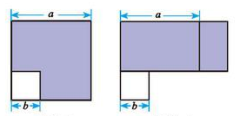
\includegraphics[width=0.5\linewidth]{pic/20200429004.png}\\
\begin{solution}
        (1) \(a^2 -b^2\)\\
        (2) 长:\((a+b)\),宽\((a-b)\),面积\((a+b)(a-b)\)\\
        (3) \(a^2 -b^2=(a+b)(a-b)\)
\end{solution}
\end{liti}

\paragraph{平方差公式应用}%
\label{par:平方差公式应用}
\begin{liti}[resume]
\item
    \begin{liti}
    \item 计算下列算式,并观察它们共同的特点
        \begin{multicols}{3}
            \begin{liti}[resume]
            \item \(7\times 9=\)  \tkt{\(63\)}
            \item \(8\times 8=\)  \tkt{\(64\)}
            \item \(11\times 13=\)  \tkt{\(143\)}
            \item \(12\times 12=\)  \tkt{\(144\)}
            \item \(79 \times 81=\)  \tkt{\(6399\)}
            \item \(80 \times 80=\)  \tkt{\(6400\)}
            \end{liti}
        \end{multicols}
    \item 用字母表示这一规律.  \tkt{\((n+1)(n-1)=n^2-1\)}
    \end{liti}
\item 用平方差公式进行计算:
    \begin{liti}
    \item \(103\times 97\) = \tkt{\(9991\)}
    \item \(118\times 122\) = \tkt{\(14436\)}
    \end{liti}
\item 计算:
    \begin{liti}
    \item \(a^2(a+b)(a-b)+a^2b^2\) = \tkt{\(a^4\)}
    \item \((2x-5)(2x+5)-2x(2x-3)\) = \tkt{\(4x^2-25-4x^2+6x=6x-25\)}
    \item \(704\times 696\) = \tkt{\(700^2-4^2=489984\)}
    \item \((x+2y)(x-2y)+(x+1)(x-1)\) = \tkt{\(x^2-4y^2+x^2-1=2x^2-4y^2-1\)}
    \item \(x(x-1)-(x-\frac{1}{3})(x+\frac{1}{3})\) = \tkt{\(x^2-x-x^2+\frac{1}{9}=-x+\frac{1}{9}\)}
    \end{liti}
\end{liti}

\subsubsection{习题}%
\label{ssub:习题}

\paragraph{平方差公式}%
\begin{xiti}[resume]
\item 计算:
    \begin{xiti}
    \item \((3x+7y)(3x-7y)\) = \tkt{\(9x^2-49y^2\)}
    \item \((0.2x-0.3)(0.2x+0.3)\) = \tkt{\(0.04x^2-0.09\)}
    \item \((mn-3n)(mn+3n)\) = \tkt{\(m^2n^2-9n^2\)}
    \item \((-2x+3y)(-2x-3y)\) = \tkt{\(4x^2-9y^2\)}
    \item \((-\frac{1}{4}x-2y)(-\frac{1}{4}x+2y)\) = \tkt{\(\frac{1}{16}x^2-4y^2\)}
    \item \((5m-n)(-5m-n)\) = \tkt{\(n^2-25m^2\)}
    \end{xiti}
\item 计算:
    \begin{xiti}
    \item \((a^n+b)(a^n-b)\) = \tkt{\(a^{2n}-b^2\)}
    \item \((a+1)(a-1)(a^2+1)\) = \tkt{\(a^4-1\)}
    \end{xiti}
\end{xiti}

\paragraph{平方差公式应用}%
\begin{xiti}[resume]
\item 计算:
    \begin{liti}
    \item \((2m+3)(2m-3)\) = \tkt{\(4m^2-9\)}
    \item \(x(x+1)+(2-x)(2+x)\) = \tkt{\(x^2+x+4-x^2=x+4\)}
    \item \((3x-y)(3x+y)+y(x+y)\) = \tkt{\(9x^2-y^2+xy+y^2=9x^2+xy\)}
    \item \((a+\frac{1}{2}b)(a-\frac{1}{2}b)-(3a-2b)(3a+2b)\) = \tkt{\(a^2-\frac{1}{4}b^2-9a^2+4b^2=-8a^2+\frac{15}{4}b^2\)}
    \end{liti}
\item 用平方差公式进行计算:
    \begin{liti}
    \item \(1007\times 993\) = \tkt{\(1000^2-49=999,951\)}
    \item \(108\times 112\) = \tkt{\(110^2-4=12096\)}
    \end{liti}
\end{xiti}

\section{完全平方公式}%

\subsubsection{知识要点}%
\label{ssub:知识要点}

\begin{enumerate}
    \item 公式:
        \begin{equation}
            (a \pm b)^2 = a^2 \pm 2ab + b^2
        \end{equation}

    \item 公式推导
        \begin{eqnarray}
            (a+b)^2=(a-b)(a-b)=a^2-2ab+b^2 \notag \\
            (a-b)^2=[a+(-b)]^2=a^2+2a(-b)+(-b)^2=a^2-2ab+b^2 \notag
        \end{eqnarray}
    \item 应用:因式分解,简便计算
\end{enumerate}

\subsubsection{例题}%
\label{ssub:例题}

\begin{liti}[resume]
\item 计算:
    \begin{liti}
    \item \((m+3)^2\) = \tkt{\(m^2+6m+9\)}
    \item \((2+3x)^2\) = \tkt{\(9x^2+12x+4\)}
    \end{liti}
\item 用下图解释和验证完全平方公式:\\
    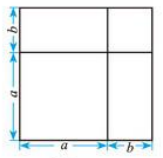
\includegraphics[width=0.3\linewidth]{pic/20200429005.png}\\
\item 利用完全平方公式计算:
    \begin{liti}
    \item \((2x-3)^2\) = \tkt{\(4x^2-12x+9\)}
    \item \((4x+5y)^2\) = \tkt{\(16x^2+40xy+25y^2\)}
    \item \((mn-a)^2\) = \tkt{\(m^2n^2-2a mn+a^2\)}
    \end{liti}
\item 计算:
    \begin{liti}
    \item \((\frac{1}{2}x-2y)^2\) = \tkt{\(\frac{1}{4}x^2-xy+4y^2\)}
    \item \((2xy+\frac{1}{5}x)^2\) = \tkt{\(4x^2y^2+\frac{4}{5}x^2y+\frac{1}{25}x^2\)}
    \item \((n+1)^2-n^2\) = \tkt{\(n^2+2n+1-n^2=2n+1\)}
    \end{liti}
\item 计算:
    \begin{liti}
    \item \(102^2 \) = \tkt{\((100+2)^2=10000+400+4=10404\)}
    \item \(197^2\) = \tkt{\((200-3)^2=200^2-1200+9=38809\)}
    \end{liti}

\item 计算:
    \begin{liti}[resume]
    \item \((x+3)^2-x^2\) = \tkt{\(6x+9\)}
    \item \((a+b+3)(a+b-3)\) = \tkt{\((a+b)^2-9=a^2+2ab+b^2-9\)}
    \item \((x+5)^2-(x-2)(x-3)\) = \tkt{\(x^2+10x+25-(x^2-5x+6)=15x+19\)}
    \end{liti}
\item 一位老人非常喜欢孩子,每当有孩子到他家做客时,老人都要拿出糖果招待他们.如果来一个孩子,老人就给这个孩子1块糖;来两个孩子,老人就给每个孩子2块糖,如果来3个孩子,老人就给每个孩子3块糖果\(\cdots\cdots\)\\
    假如第一天有a个孩子一起去看老人,第二天有b个孩子一起去看老人,第三天有\((a+b)\)个孩子一起去看老人,那么第三天老人给出去的糖果和前两天给出去的糖果总数一样多吗?
\begin{solution}
        第一天:\(a^2 \),第二天:\(b^2 \),第三天:\((a+b)^2\)\\
\end{solution}
\item 利用整式乘法公式计算:
    \begin{liti}[resume]
    \item \(96^2\) = \tkt{\((100-4)^2=9216\)}
    \item \((a-b-3)(a-b+3)\) = \tkt{\((a-b)^2-3^2=a^2-2ab+b^2-9\)}
    \end{liti}
\end{liti}

\subsubsection{习题}%
\label{ssub:习题}
\begin{xiti}[resume]
\item 计算:
    \begin{xiti}
    \item \((2x+5y)^2\) = \tkt{\(4x^2+20xy+25y^2\)}
    \item \((\frac{1}{3}m-\frac{1}{2})^2\) = \tkt{\(\frac{1}{9}m^2-\frac{1}{3}m+\frac{1}{4}\)}
    \item \((-2t-1)^2\) = \tkt{\(4t^2+4t+1\)}
    \item \((\frac{1}{5}x+\frac{1}{10}y)^2\) = \tkt{\(\frac{1}{25}x^2+\frac{1}{25}xy+\frac{1}{100}y^2\)}
    \item \((7ab+2)^2\) = \tkt{\(49a^2b^2+28 ab+4\)}
    \item \((-cd+\frac{1}{2})^2\) = \tkt{\(c^2d^2-cd+\frac{1}{4}\)}
    \end{xiti}
\item 一个圆的半径长为\(r \, cm\),减少\(2 \,\)cm后,这个圆的面积减少了多少?
\begin{solution}
        \(\pi r^2 - \pi (r-2)^2 = (4\pi r-4\pi ) \squaren{\centi\metre }\)\\
\end{solution}
\item 观察下列各式:\(15^2 =225,25^2=625,35^2=1225, \cdots\)\\
    个位数字是5的两位数平方后,末尾的两个数有什么规律?为什么?
\begin{solution}
        末尾都是25. \((10 n + 5)^2=100 n^2 + 100 n + 25=100 n(n+1)=25\)\\
\end{solution}
\item 计算\((a+b+c)^2\)
\begin{solution}
        \((a+b)^2+2(a+b)c + c^2=a^2+2ab+b^2+2ac+2bc+c^2=a^2+b^2+c^2+2ab+2bc+2ac\)\\
\end{solution}
\item 计算:
    \begin{xiti}
    \item \((2x+y+1)(2x+y-1)\) = \tkt{\((2x+y)^2-1=4x^2+4xy+y^2-1\)}
    \item \((x-2)(x+2)-(x+1)(x-3)\) = \tkt{\(x^2-4-(x^2-2x-3)=2x-1\)}
    \item \((ab+1)^2-(ab-1)^2\) = \tkt{\((ab+1+ab-1)(ab+1-ab+1)=4ab\)}
    \item \((2x-y)^2-4(x-y)(x+2y)\) = \tkt{\(4x^2-4xy+y^2-4(x^2+xy-2y^2)=-8xy+9y^2\)}
    \end{xiti}
\item 一个底面是正方形的长方体,高为\(6 \, cm\),底面正方形边长为\(5 \, cm\),如果它的高不变,底面正方形边长增加了\(a \, cm\),那么它的体积增加了多少?
\begin{solution}
        原体积: \(6\times 5\times 5=150\); 改变后体积 \(6\times (5+a)(5+a)=6a^2+60a+150\)\\
        所以,增加\(6a^2+60a\)
\end{solution}
\item 利用完全平方公式计算:
    \begin{xiti}
    \item \(63^2 \) = \tkt{\((60+3)^2=3600+360+9=3969\)}
    \item \(998^2 \) = \tkt{\((1000-2)^2=1000^2-4\times 1000+4=996004\)}
    \end{xiti}
\item 计算\((a+b)^3\)
\begin{solution}
        \(=(a+b)^2(a+b)=(a^2+2ab+b^2)(a+b)=a^3+3a^2b+3ab^2+b^3\)\\
\end{solution}
\end{xiti}

\section{整式的除法}%
\label{sec:整式的除法}
\subsubsection{知识要点}%
\label{ssub:知识要点}
\begin{enumerate}
    \item 单项式相除:把系数,同底数幂分别相除后,作为商的因式;对于只在被除式里含有的字母,则连同它的指数一起作为商的一个因式.\\
        \(x^5y \div x^2; 8m^2n^2 \div 2m^2n; a^4b^2c \div 3a^2b\)
    \item 多项式除以单项式,先把多项式的每一项分别除以单项式,再把所得的商相加.\\
        \((ad+bd)\div d; (a^2b+3ab) \div a; (xy^3-2xy) \div xy\)
    \item 类比分数约分
\end{enumerate}

\subsubsection{例题}%
\label{ssub:例题}

\paragraph{单项式除单项式}%

\begin{liti}[resume]
\item 计算:
    \begin{liti}
    \item \(-\frac{3}{5}x^2y^3 \div 3x^2y\) = \tkt{\(-\frac{1}{5}y^2\)}
    \item \(10a^4b^3c^2 \div 5a^3bc\) = \tkt{\(2ab^2c\)}
    \item \((2x^2y)^3 \cdot (-xy^2) \div 14x^4y^3\) = \tkt{\(-\frac{4}{7}x^3y^2\)}
    \item \((2a+b)^4 \div (2a+b)^2\) = \tkt{\((2a+b)^2=4a^2+4ab+b^2\)}
    \end{liti}
\item 如图,三个大小相同的球恰好放在一个圆柱形盒子里,三个球的体积之和占整个盒子容积的几分之几?\\
    
\includegraphics[width=0.1\linewidth]{pic/20200429006.png}\\
\begin{solution}
        三个球体积= \(3\times \frac{4}{3}\pi r^3=4\pi r^3\); 圆柱体积=\(Sh=\pi r^2 \cdot 6r=6\pi r^3\); \(\frac{4\pi r^3}{6\pi r^3}=\frac{2}{3}\)\\
\end{solution}
\item 计算:
    \begin{liti}
    \item \(2a^6b^3 \div a^3b^2\) = \tkt{\(2a^3b\)}
    \item \(\frac{1}{48}x^3y^2 \div \frac{1}{16}x^2y\) = \tkt{\(\frac{1}{3}xy\)}
    \item \(3m^2n^3 \div (mn)^2\) = \tkt{\(3n\)}
    \item \((2x^2y)^3 \div 6x^3y^2\) = \tkt{\(\frac{4}{3}x^3y\)}
    \end{liti}
\end{liti}

\paragraph{单项式除多项式}%
\begin{liti}[resume]
\item 计算:
    \begin{liti}
    \item \((6ab+8b)\div 2b\) = \tkt{\(3a+4\)}
    \item \((27a^3-15a^2+6a) \div 3a\) = \tkt{\(9a^2-5a+2\)}
    \item \((9x^2y - 6xy^2) \div 3xy\) = \tkt{\(3x-2y\)}
    \item \((3x^2y - xy^2 +\frac{1}{2}xy) \div (-\frac{1}{2}xy)\) = \tkt{\(-6x+2y-1\)}
    \end{liti}
\item 小明在爬一小山时,第一阶段的平均速度为\(v\),所用时间为\(t_1\); 第二阶段的平均速度为\(\frac{1}{2}v\),所用时间为\(t_2\).\\
    下山时,小明的平均速度保持为\(4v\).已知小明上山的路程和下山的路程是相同的,那么小明下山用了多长时间?
\begin{solution}
        总路程=\(vt_1+\frac{1}{2}vt_2\), 时间=\(\frac{vt_1+\frac{1}{2}vt_2}{4v}=\frac{2t_2+t_2}{8}\)\\
\end{solution}
\end{liti}

\subsubsection{习题}%
\label{ssub:习题}

\paragraph{单项式除单项式}%
\begin{xiti}[resume]
\item 计算:\\
    \begin{xiti}
    \item \((-2r^2s)^2 \div 4rs^2\) = \tkt{\(r^3\)}
    \item \((5x^2y^3)^2 \div 25x^4y^5\) = \tkt{\(y\)}
    \item \((x+y)^3 \div (x+y)\) = \tkt{\(x^2+2xy+y^2\)}
    \item \(7a^5b^3c^5 \div 14a^2b^3c\) = \tkt{\(\frac{1}{2}a^3c^4\)}
    \end{xiti}
\item 计算:\\
    \begin{xiti}
    \item \(8a^4b^3c \div 2a^2b^3 \cdot (-\frac{2}{3}a^3bc^2)\) = \tkt{\(-\frac{8}{3}a^5bc^3\)}
    \item \((3x^2y)^2\cdot (-15xy^3)\div (-9x^4y^2)\) = \tkt{\(15xy^3\)}
    \end{xiti}
\item 我们都知道``先看见闪电,后听见雷声'',那是因为在空气中光的传播速度比声音快,科学家们发现,光在空气中的传播速度约为\(3 \times 10^8m/s\),而声音在空气中的传播速度大约只有\(300m/s\),你能进一步算出光的传播速度是声音的多少倍吗?
\begin{solution}
        \(3\times 10^8 \div 300 = 10^6\)倍\\
\end{solution}

\item 一个圆柱形桶装满了水,已知桶的底面直径为\(a\),高为\(b\).又知另一长方体形容器的长为\(b\),宽为\(a\),若把圆柱形桶中水倒入长方体形容器中(水不溢出),水面高度是多少?
\begin{solution}
        \(\pi \times (\frac{a}{2})^2 \times b \div (ab)=\frac{1}{4}\pi a^2b \times \frac{1}{ab}=\frac{1}{4}\pi a\)\\
\end{solution}
\end{xiti}

\paragraph{多项式除单项式}%
\begin{xiti}[resume]
\item 计算:\\
    \begin{xiti}
    \item \((5m^3n^2-6m^2)\cdot 3m\) = \tkt{\(\frac{5}{3}m^2n^2 -2m\)}
    \item \((6a^2b-5a^2c^2)\div (-3a^2)\) = \tkt{\(-2b+\frac{5}{3}c^2\)}
    \item \((16x^4+4x^2+x)\div x\) = \tkt{\(16x^3+4x+1\)}
    \item \((3a^2b-2ab+2ab^2)\div ab\) = \tkt{\(3a-2+2b\)}
    \item \((-4a^3+6a^2b^3+3a^3b^3)\div (-4a^2)\) = \tkt{\(a-\frac{3}{2}b^3-\frac{3}{4}ab^3\)}
    \item \((\frac{2}{5}mn^3-m^2n^2+\frac{1}{6}n^4)\div \frac{2}{3}n^2\) = \tkt{\(\frac{3}{5}mn-\frac{3}{2}m^2+\frac{1}{4}n^2\)}
    \item \((\frac{1}{10}xy^2+\frac{1}{4}y^2-\frac{1}{2}y)\div \frac{1}{5}y\) = \tkt{\(\frac{1}{2}xy+\frac{5}{4}y-\frac{5}{2}\)}
    \item \([(x+1)(x+2)-2]\div x\) = \tkt{\(x+3\)}
    \end{xiti}
\item 图(1)中的瓶子中装满了水,如果将这个瓶子中的水全部倒入图(2)的杯子中,那么一共需要多少个这样的杯子?(单位:\(cm\))\\
    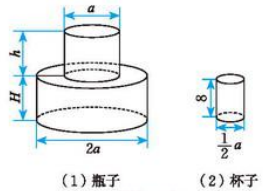
\includegraphics[width=0.3\linewidth]{pic/20200429007.png}\\
\begin{solution}
        \(V_1 = \pi (\frac{a}{2})^2h + \pi a^2 H; \quad V_2 = \pi (\frac{a}{4})^2 \times 8 = \frac{a^2}{2} \pi  \quad \frac{V_1}{V_2}=\frac{h}{2}+2H\)  \\
\end{solution}
\item 任意给一个非零数,按下列程序进行计算,写出输出结果.\\
    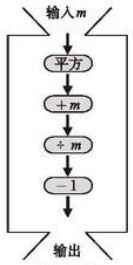
\includegraphics[width=0.15\linewidth]{pic/20200429008.png}\\
\begin{solution}
        \(m\ne 0, (m^2+m)\div m-1=m\)\\
\end{solution}
\end{xiti}
\section{章总结}%
\label{sec:章总结}

\subsubsection{知识要点}%
\label{ssub:知识要点}

\begin{enumerate}
    \item 同底数幂的乘法:底数不变,指数相加.\(a^m \cdot a^n = \tkt{a^{m+n}}, \, a^m \cdot a^n \cdot a^p = \tkt{a^{m+n+p}}\);
    \item 幂的乘方: 运算规则:同底数幂的乘方,底数不变,指数相乘.  \((a^m)^n = \)\tkt{\(a^{mn}\)}
    \item 积的乘方: 积的乘方等于\tkt{乘方的积}. \((ab)^n = \)\tkt{\(a^nb^n\)}
    \item 同底数幂的除法:同底数幂相除,底数不变,指数相减. \(a^m \div  a^n = \)\tkt{\(a^{m-n}\)}, \quad \(a^0=1(a\ne 0)\), \quad \(a^{-p}=\frac{1}{a^p}(a\ne 0)\)
    \item 科学记数法:把一个数表示成\(a\)与\(10\)的\(n\)次幂相乘的形式\((1\le |a|<10,n\)为整数),当数的绝对值小于1时,n是负整数.
    \item 整式乘法
        \begin{enumerate}
            \item 单项式与单项式相乘:把系数,相同字母的幂分别相乘,其余字母连同它的指数不变作为积的因式.\(2xy\cdot 3x^2y^2z=6x^3y^3z\)
            \item 单项式与多项式相乘:根据分配率用单项式去乘多项式的每一项,再把所得的积相加.\(m(a+b+c)=ma+mb+mc\)
            \item 多项式与多项式相乘:先用一个多项式的每一项乘另一个多项式的每一项,再把所得的积相加.\((a+b)(m+n)=am+an+bm+bn\)
        \end{enumerate}
    \item 平方差公式: \((a+b)(a-b)=a^2-b^2\)
    \item 完全平方公式:\((a \pm b)^2 = a^2 \pm 2ab + b^2\)
    \item 整式除法:类比分数约分
        \begin{enumerate}
            \item 单项式相除:把系数,同底数幂分别相除后,作为商的因式;对于只在被除式里含有的字母,则连同它的指数一起作为商的一个因式.如: \(8m^2n^2 \div 2m^3np = \frac{4n}{mp}\)
            \item 多项式除以单项式,先把多项式的每一项分别除以单项式,再把所得的商相加.如: \( (a^2b+3ab) \div a = ab + 3b \)
        \end{enumerate}
\end{enumerate}


\subsubsection{例题}%

\begin{liti}[resume]
\item 概念巩固:整式,单项式,多项式,乘方,幂,底数,指数
\item 同底数幂相乘.口算:
    \begin{liti}
    \item \(a \cdot a^3 \cdot a^5\)\tkt{\(=a^9\)}
    \item \((-b)^2(-b)^3(-b)^5\) \tkt{\(=b^{10}\)}
    \item \((m+n)^2(m+n)^3\)\tkt{\(=(m+n)^5\)}
    \item \((x-2y)^2(2y-x)^3\) \tkt{\(=(2y-x)^5\)}
    \end{liti}
\begin{note}
        技巧: \((a-b)^n = \begin{cases} (b-a)^n & n\text{为偶数}\\ -(b-a)^n & n\text{为奇数}\\  \end{cases}\)
\end{note}
\item 幂的乘方.口算
    \begin{liti}
    \item \((-11^2)^3=\)\tkt{\(-11^6\)}
    \item \((-11^3)^2=\)\tkt{\(11^6\)}
    \item \([(-x^3)]^4=\)\tkt{\(x^{12}\)}
    \item \((a^3)^2\cdot (a^2)^3=\)\tkt{\(a^{12}\)}
    \item \((y^3)^6-(y^2)^9=\)\tkt{\(0\)}
    \item \((x^{2m-2})^4\cdot (x^{m+1})^2=\)\tkt{\(x^{10 m-6}\)}
    \item \([(a-b)^2]^3 \cdot [(b-a)^3]^3 =\)\tkt{\( (b-a)^{15}\)}
    \item \([(-a)^3]^4 + [(-a)^6]^2 =\)\tkt{\( 2a^{12}\)}
    \item \([(-2)^3]^3 + [(-2^5)]^5 =\)\tkt{\( -2^9 + 2^{10}=2^9\)}
\begin{note}
            易错题,需化简到最简形式
\end{note}
    \end{liti}
\item 积的乘方.口算
    \begin{liti}
    \item \((3x^4)^2=\)\tkt{\(9x^8\)}
    \item \((2a^3b)^2=\)\tkt{\(4a^6b^2\)}
    \item \((-1\frac{1}{2}xy^2z^2)^3=\)\tkt{\(-\frac{27}{8}x^3y^6z^6\)}
    \item \((-a^mb^{3m})^2=\)\tkt{\(a^{2m}b^{6m}\)}
    \item \((2\times 10^2)^3\times (-10^3)^4=\)\tkt{\(8\times 10^{18}\)}
    \item \([3(a+b)^2]^3[-2(a+b)^3]^2=\)\tkt{\(108(a+b)^{12}\)}
    \end{liti}
\item 找出下列式子中的单项式,多项式和分式:\\
    \(a^2-1,0,\frac{1}{3a},x+\frac{1}{y},-\frac{xy^2}{4},m,\frac{x+y}{2},\sqrt{2}-3b\)
\begin{solution}
        单项式:\(0,-\frac{xy^2}{4},m,\)\\
        多项式:\(a^2-1,\frac{x+y}{2},\sqrt{2}-3b\)\\
        分式: \(\frac{1}{3a},x+\frac{1}{y}\)
\end{solution}
\item 概念巩固:如何确定单项式的次数\\
    \(\frac{-3 \times 10^2\pi a^5b}{4}\)
\item 概念巩固:如何确定多项式的次数与项数.\\
    \(10^5a^2b+a^5b^{11}-7ab\cdot 3+6a\) \tkt{16次3项式}
\item \(3x^{7-m}y^{n+3}\text{与}-4x^{1-4m}y^{2n}\)是同类项,求\(m,n\)\\
\begin{solution}
        \(7-m=1-4m, n+3=2n \Rightarrow m=-2,n=3\)
\end{solution}
\item 单项式乘单项式.口算
    \begin{liti}
    \item \(10x^2yz^3(-\frac{1}{2}xy^4)=\)\tkt{\(-5x^3y^5z^3\)}
    \item \((-\frac{3}{7}ab^2)(\frac{7}{3}a^2bc)=\)\tkt{\(-a^3b^3c\)}
    \item \(3ab^2(-\frac{1}{3}a^2b)2abc=\)\tkt{\(-2a^4b^4c\)}
    \item \((-2x^{n+1}y^n)(-3xy)(-\frac{1}{2}x^2z)=\)\tkt{\(-3x^{n+4}y^{n+1}z\)}
    \item \(-6a^2b(x-y)^2\cdot \frac{1}{3}ab^2(y-x)^2=\)\tkt{\(-2a^3b^3(x-y)^5\)}
    \item \(-\frac{3}{5}(m+n)^3\cdot n \cdot \frac{4}{3}(m+n)p=\)\tkt{\(-\frac{4}{5}(m+n)^4np\)}
    \end{liti}
\item \(\frac{\sqrt{15-2x^2}}{3}\)是单项式还是多项式?是整式吗?
\item 单项式乘多项式.
    \begin{liti}
    \item \(-\frac{3}{2}xy(\frac{2}{3}x^2y-4xy^2+\frac{4}{3}y)=\)\tkt{\(-x^3y^2+6x^2y^3-2xy^2\)}
    \item \(6mn^2(2-\frac{1}{3}mn^4)=\)\tkt{\(12mn^2-2m^2n^6\)}
    \item \(-3a^2b(9ab^2+2a^2b-3abc)=\)\tkt{\(-27a^3b^3-6a^4b^2+9a^3b^2c\)}
    \end{liti}
\item 多项式乘多项式
    \begin{liti}
    \item \((x+y)(a+b)=\)\tkt{\(ax+bx+ay+by\)}
    \item \((x-y)(x+y)=\)\tkt{\(x^2-y^2\)}
    \item \((x-2)(x^2+4x-3)=\)\tkt{\(x^3+2x^2-11x+6\)}
    \item \((x-3)(3x+4)=\)\tkt{\(3x^2-5x-12\)}
    \item \((4x-3y)(4x+3y)=\)\tkt{\(16x^2-9y^2\)}
    \end{liti}

\item 同底数幂相除.
    \begin{liti}
    \item \(-a^4\div a=\)\tkt{\(-a^3\)}
    \item \(5^8 \div 5^6=\)\tkt{\(25\)}
    \item \(a^4b^4 \div (ab)^2=\)\tkt{\(a^2b^2\)}
    \end{liti}
\item 单项式除单项式.
    \begin{liti}
    \item \(6x^2y \div 3xy=\)\tkt{\(2x\)}
    \item \(-8a^2b^3 \div 6ab^2=\)\tkt{\( -\frac{4}{3}ab\)}
    \item \(4a^3b^4 \div 2a^3b =\)\tkt{\( 2b^3\)}
    \end{liti}
\item 多项式除单项式.
    \begin{liti}
    \item \((25x^2-20x^4) \div (-5x^2) =\)\tkt{\( -5 + 4x^2\)}
    \item \(\frac{-4a^3+12a^2b-7a^3b^2}{-4a^2}=\)\tkt{\(a-3b+\frac{7}{4}ab^2\)}
    \end{liti}
\item 平方差公式.
    \begin{liti}
    \item 用语言描述平方差公式
    \item \((xy+1)(xy-1)=\)\tkt{\(x^2y^2-1\)}
    \item \((ab+cd)(ab-cd)=\)\tkt{\(a^2b^2-c^2d^2\)}
    \item \((2a+3)(2a-3)=\)\tkt{\(4a^2-9\)}
    \item \((x^2+yz)(x^2-yz)=\)\tkt{\(x^4-y^2z^2\)}
    \item \((a+3)(a-3)-(a+4)(a-4)=\)\tkt{\(7\)}
    \item \((x-3)(x^2+9)(x+3)=\)\tkt{\(x^4-81\)}
    \item \(100.5 \times 99.5 =\)\tkt{\( 9999.75\)}
    \end{liti}
\item 完全平方公式
    \begin{liti}
    \item 用语言描述完全平方公式
    \item \(x^2-16x+64=\)\tkt{\((x-8)^2Ï\)}
    \item \(x^2+6x+\)\tkt{\(9\)}=\tkt{\((x+3)^2\)}
    \item \(x^2+8x+\)\tkt{\(16\)}=\tkt{\((x+4)^2\)}
    \item \(x^2-20x+\)\tkt{\(100\)}=\tkt{\((x-10)^2\)}
    \item \(x^2+40x+\)\tkt{\(400\)}=\tkt{\((x+20)^2\)}
    \item \((3a+b)^2=\)\tkt{\(9a^2+6ab+b^2\)}
    \item \((x-2y)^2=\)\tkt{\(x^4-4xy+4y^2\)}
    \item \((3a+b)^2=\)\tkt{\(9a^2+6ab+b^2\)}
    \item \((x-2y)^2=\)\tkt{\(x^2-4xy+4y^2\)}
    \item \((-2x-3y)^2=\)\tkt{\(4x^2+12xy+9y^2\)}
    \item \(2002^2=\)\tkt{\(4008004\)}
    \item \(1999^2=\)\tkt{\(3996001\)}
    \end{liti}
\item 判断正误:
    \begin{liti}
    \item \(a^3+a^3=a^6\)  \tkt{\(=2a^3\)}
    \item \((3a^3)^2=6a^6\) = \tkt{\(9a^6\)}
    \item \(a^3a^3=a^6\) = \tkt{\ding{51}}
    \item \((a^3)^3=a^6\) = \tkt{\(=a^9\)}
    \item \(1-\frac{1}{4}x^2=\frac{1}{4}(x+2)(x-2)\) = \tkt{\(=\frac{1}{4}(2+x)(2-x)\)}
    \item \((x-y)^3-(y-x)=(x-y)(x-y+1)(x-y-1)\) = \tkt{\(=(x-y)[(x-y)^2+1]\)}
    \item \(4x-2x^2-2=-2(x-1)^2\)  = \tkt{\(=-2[(x-1)^2+1]\)}
    \item \(x^2 -y^2-x+y=(x+y)(x-y-1)\) = \tkt{\(=(x-y)(x+y-1)\)}
    \end{liti}
\item 逆用幂运算:
    \begin{liti}
    \item \(2^m=64,2^n=8,\text{求}2^{m+n}\)
\begin{solution}
            \(2^{m+n}=2^m\cdot 2^n=64\times 8=512\)\\
\end{solution}
    \item \((-2)^{2007} + (-2)^{ 2008 }\)
\begin{solution}
            \(=-2^{2007}+2^{2008}=2^{2007}\)\\
\end{solution}
    \end{liti}
\item 逆用幂乘方:\(a=2^{555}, b=3^{444}, c=5^{333}\), 比较\(a,b, c \)的大小
\begin{solution}
        \(a=(2^5)^{111}=32^{111}, b=81^{111}, c=125^{111}, \therefore a<b<c\)\\
\end{solution}
\item 逆用积的乘方: 求\((\frac{99}{100})^{2008} \times (\frac{100}{99})^{2009}\)
\begin{solution}
        原式\(= (\frac{99}{100})^{2008} \times (\frac{100}{99})^{2008} \times \frac{100}{99}=(\frac{99}{100} \times \frac{100}{99})^{2008} \times \frac{100}{99}=\frac{100}{99}\)\\
\end{solution}
\item 逆用同底数幂相除:已知\(5^m=3,25^m=11,\text{求}5^{3m-2n}\)
\begin{solution}
        \(5^{3m-2n}=\frac{5^{3m}}{5^{2n}}=\frac{(5^m)^3}{25^n}=\frac{27}{11}\)\\
\end{solution}
\item 灵活运用整式乘法
    \begin{liti}
    \item 已知\(xy^2=-6, \text{求} -xy(x^3y^7-3x^2y^5-5y)\)
\begin{solution}
            原式=\(-x^4y^8 + 3x^3y^6 + 5xy^2 = -(xy^2)^4 + 3(xy^2)^3 + 5xy^2 = -(-6)^4 +3(-6)^3 +5\times (-6)=1974\)\\
\end{solution}
    \item 已知\(x^2 - 5x=6, \text{求} (x-1)(x-2)(x-3)(x-4)\)
\begin{solution}
            原式=\([(x-1)(x-4)(x-2)(x-3)=(x^2-5x+4)(x^2-5x+6)=120\)\\
\end{solution}
    \end{liti}
\item 指数方程求解:
    \begin{liti}
    \item \(4^{3x-1} \times 16 = 64 \times 4, \text{求}x\)
\begin{solution}
            原式变化: \(4^{3x-1} = 16 \Rightarrow 3x-1=2 \Rightarrow x=1\)\\
\end{solution}
    \item 已知\(a^{n+1}\cdot a^{m+2}=a^7,\text{且}m-2n=1\),求\(m^n\)
\begin{solution}
            \(a^{m+n+3}=a^7 \Rightarrow m+n=4, \text{又}m-2n=1 \Rightarrow m=3,n=1, m^n=3\)\\
\end{solution}
    \end{liti}
\item 熟练运用两个公式:下列哪些式子可以用平方差公式,哪些式子可以用完全平方公式.
    \begin{liti}
    \item \((a+b)(a-b) =\)\tkt{\( a^2-b^2\)}
    \item \((-a+b)(-a-b)=\)\tkt{\(a^2-b^2\)}
    \item \((-a-b)(a-b)=\)\tkt{\(b^2-a^2\)}
    \item \((-a-b)(-a+b)=\)\tkt{\(a^2-b^2\)}
    \item \((-a-b)(a+b)=\)\tkt{\(-a^2-2ab-b^2\)}
    \item \((-a+b)(a-b)=\)\tkt{\(-a^2+2ab-b^2\)}
    \item \((x-3)(x^2+9)(x+3)=\)\tkt{\(x^4-81\)}
    \item \((2y-x-3z)(-x-2y-3z)=\)\tkt{\((x+3z)^2-4y^2=x^2+6xz+9z^2=4y^2\)}
    \item \((1-\frac{1}{2^2})(1-\frac{1}{3^2})(1-\frac{1}{4^2})\cdots(1-\frac{1}{10^2})\)
\begin{solution}
            原式=\((1+\frac{1}{2})(1-\frac{1}{2})(1+\frac{1}{3})(1-\frac{1}{3}) \cdots (1+\frac{1}{10})(1-\frac{1}{10})=\frac{1}{2}\times \frac{3}{2} \times \frac{2}{3} \times \frac{4}{3}\times \frac{4}{3}\times \frac{5}{4} \cdots \frac{9}{10} \times \frac{11}{10}=\frac{1}{2}\times \frac{11}{10}=\frac{11}{20}\)\\
\end{solution}
    \end{liti}
    \end{liti}

    \subsubsection{习题}%
    \label{ssub:习题}

    \begin{xiti}[resume]
    \item 计算:
        \begin{multicols}{2}
            \begin{xiti}
            \item \((-\frac{3}{5})^2\cdot (-\frac{3}{5})^3\) \tkt{\(=(-\frac{3}{5})^5=-\frac{243}{1725}\)}
            \item \((a-b)^3\cdot (a-b)^4\) \tkt{\(=(a-b)^7\)}
            \item \((-a^5)^5\) \tkt{\(=-a^{25}\)}
            \item \((-\frac{1}{2}x)^7 \div (-\frac{1}{2}x)\) \tkt{\(=\frac{1}{64}x^6\)}
            \item \((a+b)^3 \div (a+b)\) \tkt{\(=(a+b)^2\)}
            \item \( (-a^2 \cdot b)^3\) \tkt{\(=-a^6b^3\)}
            \item \((-a)^2(a^2)^2\) \tkt{\(=a^6\)}
            \item \((y^2)^3 \div y^6\) \tkt{\(=1\)}
            \item \((-y)^2 \cdot y^{n-1} (n>1)\) \tkt{\(=y^{n+1}\)}
            \item \(a^{n+1} \cdot a^{n-1}(n>1)\) \tkt{\(=a^{2n}\)}
            \item \(a^{m+2} \div a^{m+1}\) \tkt{\(=a\)}
            \item \((-c^2)^{2n}\) \tkt{\(=c^{4n}\)}
            \end{xiti}
        \end{multicols}
    \item 计算:
        \begin{xiti}
        \item \(10^5 \div 10^{-1} \times 10^0\) \tkt{\(=10^6\)}
        \item \(16 \times 2^{-4}\) \tkt{\(=1\)}
        \item \((\frac{1}{3})^0 \div (-\frac{1}{3})^{-2}\) \tkt{\(=-9\)}
        \end{xiti}
    \item 一个正方体的棱长为\(2\times 10^2 \, mm\).\\
        (1)它的表面积是多少平方米?\\
        (2)它的体积是多少立方米?
\begin{solution}
            (1) 边长\(a= 0.2m, S= 0.2 \times 0.2 \times 6 = 0.24 \squaremetre \)\\
            (2) 体积\(V=0.2\times 0.2\times 0.2=0.008 \cubic\metre \)
\end{solution}
    \item 计算:
        \begin{xiti}
        \item \((x+a)(x+b)\) \tkt{\(=x^2 + ax + bx + ab\)}
        \item \((3x+7y)(3x-7y)\) \tkt{\(=9x^2-49y^2\)}
        \item \((3x+9)(6x+8)\) \tkt{\(=18x^2+78x+72\)}
        \item \((\frac{1}{2}x^2y-2xy+y^2)\cdot 3xy\) \tkt{\(=\frac{3}{2}x^3y^2-6x^2y^2+3xy^3\)}
        \item \(\frac{1}{3}a^2b^3\cdot (-15a^2b^2)\) \tkt{\(=-5a^4b^5\)}
        \item \((4a^3b-6a^2b^2+12ab^3)\div 2ab\) \tkt{\(=2a^2-3ab+6b^2\)}
        \item \((a^2bc)^2\div ab^2c\) \tkt{\(=a^3c\)}
        \item \((3mn+1)(3mn-1)-8m^2n^2\) \tkt{\(=m^2n^2-1\)}
        \item \([(3a+b)^2-b^2]\div a\) \tkt{\(= 9a+6b\)}
        \item \((x+2)^2-(x+1)(x-1)\) \tkt{\(=4x+5\)}
        \end{xiti}
    \item 计算:
        \begin{multicols}{2}
            \begin{xiti}
            \item \(10^7 \div (10^3 \div 10^2)\) \tkt{\(=10^6\)}
            \item \((x-y)^3 \cdot (x-y)^2 \cdot (y-x)\) \tkt{\(=-(x-y)^6\)}
            \item \(4 \times 2^n \times 2^{n-1}(n>1)\) \tkt{\(=2^{2n+1}\)}
            \item \((-x)^3 \cdot x^{2n-1} + x^{2n}\cdot (-x)^2\) \tkt{\(=0\)}
            \item \((y^2 \cdot y^3) \div (y\cdot y^4)\) \tkt{\(=1\)}
            \item \(x^2\cdot x^3 + x^7 \div x^2\) \tkt{\(=2x^5\)}
            \item \(m^5 \div m^2 \times m\) \tkt{\(=m^4\)}
            \item \(a^4 + (a^2)^4 -(a^2)^2\) \tkt{\(=a^8\)}
            \end{xiti}
        \end{multicols}
    \item 计算:
        \begin{xiti}
        \item \((2x^2)^3 - 6x^3(x^3+2x^2+x)\) \tkt{\(=2x^6-12x^5-6x^4\)}
        \item \((x+y+z)(x+y-z)\) \tkt{\(=x^2+2xy+y^2-z^2\)}
        \item \([(x+y)^2-(x-y)^2]\div 2xy\) \tkt{\(=2\)}
        \item \(a^2(a+1)^2-2(a^2-2a+4)\) \tkt{\(=a^4+2a^3-a^2+4a-8\)}
        \end{xiti}
    \item 求下列各式的值:
        \begin{xiti}
        \item \(3x^2+(-\frac{3}{2}x+\frac{1}{3}y^2)(2x-\frac{2}{3}y)\),其中\(x=-\frac{1}{3},y=\frac{2}{3}\)
        \item \([(xy+2)(xy-2)-2x^2y^2+4]\div xy\),其中\(x=10,y=-\frac{1}{25}\)
        \item \(x(x+2y)-(x+1)^2+2x\),其中\(x=\frac{1}{25},y=-25\).
        \end{xiti}
\begin{solution}
            (1)原式\(=xy+\frac{2}{3}xy^2-\frac{2}{9}y^3\),代入\(x=-\frac{1}{3},y=\frac{2}{3}\),原式=\(-\frac{94}{243}\)\\
            (2)原式\(=-xy=\frac{2}{5}\)\\
            (3)原式\(=2xy-1=-3\)
\end{solution}
    \item 利用整式乘法公式计算下列各题:
        \begin{multicols}{3}
            \begin{xiti}
            \item \(2001^2\)
            \item \(2001 \times 1999\)
            \item \(99^2-1\)
            \end{xiti}
        \end{multicols}
\begin{solution}
            (1) \((2000+1)^2=4004001\)\\
            (2) \((2000+1)(2000-1)=3999999\)\\
            (3) \((99+1)(99-1)=9800\)
\end{solution}
    \item 利用整式乘法公式计算:
        \begin{multicols}{3}
            \begin{xiti}
            \item \(899\times 901 +1\)
            \item \(123^2-124\times 122\)
            \end{xiti}
        \end{multicols}
\begin{solution}
            (1) 原式\(=(900+1)(900-1)+1=810000\)\\
            (2) 原式\(=123^2-(123+1)(123-1)=1\)
\end{solution}
    \item 试用直观的方法说明\((a+3)^2 \ne a^2 + 3^2(a\ne 0)\)
\begin{solution}
            边长为\(a\)与边长为\(3\)的正方形的面积和,不等于边长为\(a+3\)的正方形的面积\\
\end{solution}
    \item 某种原子质量为\(0.000,000,000,000,000,000,000,019,93g\),你能用科学计数法把它表示出来吗?科学上把这个数量的十二分之一定为1个原子质量单位,并用符号u表示,请你用科学计数法把u表示出来.
\begin{solution}
            答:\(1.993\times 10^{-23}g,\qquad 1.661\times 10^{-24}g=1.661\times 10^{-27}kg\)\\
\end{solution}
    \item 求\((2-1)(2+1)(2^2+1)(2^4+1)\cdots (2^{32}+1)+1\)的个位数字.
\begin{solution}
            原式\(=(2^2-1)(2^2+1)(2^4+1) \cdots (2^{32}+1)+1=(2^{32}-1)(2^{32}+1)+1)=2^{64}-1+1=2^{64}\)\\
            \(2^n\)的尾数依次为2,4,8,6,2,4,8,6\(\cdots\),即周期为4的重复数列,64为4的整数倍,\(\therefore \)原式尾数为6.
\end{solution}
    \end{xiti}

    \section{强化训练}%

    \subsection{基础篇一}%
    \begin{shiti}
    \item 填空%
        \begin{shiti}
        \item \((x+1)(x-1)=\)\tkt{\(x^2-1\)}
        \item \((a-b)^2=\)\tkt{\(a^2-2ab+b^2\)}
        \item \tkt{\((a+b)^2\)}\(=a^2+2ab+b^2\)
        \item \( [(-2)^3]^3=\)\tkt{\(-2^9\)}
        \item \(x^5 \div x^3 \cdot x^2 = \)\tkt{\(x^4\)}
        \item \((x-2)(x+3)=\)\tkt{\(x^2+x-6\)}
        \item \((-a-2b)^2=\)\tkt{\((a+2b)^2\)}
        \item \((x+1)(x-1)+1=\)\tkt{\(x^2\)}
        \item \(9x^4y^5 \div (-\frac{1}{4}x^3y) \div (-3y^2)^2 = \)\tkt{\(-4x\)}
        \item \((3a^2y^2)^3-2(a^3y^3)^2=\)\tkt{\(25a^6y^6\)}
        \item \((-0.5a)(\frac{1}{3}ax^2-\frac{1}{2}a^2x-a^3)=\)\tkt{\(-\frac{1}{6}a^2x^2+\frac{1}{4}a^3x+\frac{1}{2}a^4\)}
        \item 把\((a-b)^3(a-b)+(a-b)^2(a-b)^2\)化成\((a-b)^n\)的形式:\tkt{\(2(a-b)^4\)}
        \item \((3a^{n+2}+a^{n+1})\div (-\frac{1}{3}a^{n-1})\)\tkt{\(-9a^3-3a^2\)}
        \item \(x^2-4x+\)\tkt{\(4\)}=(\tkt{\(x-2\)})\(^2\)
        \item \((-a+2b)(-a-2b)=\)\tkt{\(a^2-4b^2\)}
        \item 若\((a+3b)^2=(a-3b)^2+N\),则\(N=\)\tkt{\(12ab\)}
        \item 若\(a+b=5,ab=6\),则\(a^2+b^2=\)\tkt{\(13\)}
        \item 若\(m+n=10,mn=24,\text{则}m^2+n^2=\)\tkt{\(52\)}
        \item 如果\(4x^2+mx+9\)是一个完全平方式,那么\(m=\)\tkt{\(\pm 12\)}
        \item \((2+1)(2^2+1)(2^4+1)=\)\tkt{\(=2^8-1=255\)}
        \end{shiti}
    \item 选择题
        \begin{shiti}[resume]
        \item 下列各计算中,正确的是(\qquad)\\
            \begin{tasks}(2)
                \task \(b^5 \cdot b^5 = 2b^5\)
                \task \(x^5 + x^5 = x^{10}\)
                \task \(m^2 \cdot m^3 = m^5\)
                \task \(a \cdot b^2 = a^2b^2\)
            \end{tasks}
\begin{solution}
                C\\
\end{solution}
        \item 下列多项式乘法中,正确的是(\qquad)\\
            \begin{tasks}(2)
                \task \((a+bx)(-bx+a)=a^2-b^2x\)
                \task \((a+b)(a^2+ab+b^2)=a^3-b^3\)
                \task \((-a-b)(a+b)=-a^2-2ab-b^2\)
                \task \((a-b)(a^2+2ab+b^2)=a^3-b^3\)
            \end{tasks}
\begin{solution}
                C\\
\end{solution}
        \item 一个正方形的边长增加了\( 3 cm\),面积相应增加了\(39cm^2\),则这个正方形的边长为(\qquad)\\
            \begin{tasks}(4)
                \task \( 6cm  \)\task \( 5 cm  \)\task \( 8 cm  \)\task \( 7 cm\)
            \end{tasks}
\begin{solution}
                B.\((x+3)^2-x^2=6x+9=30 \Rightarrow x=5 \centi\metre \)\\
\end{solution}
        \item 计算结果与\((a^2b^3-a^3b^2)^2\)相同的是(\qquad)\\
            \begin{tasks}(2)
                \task \(( a^2b^3+a^3b^2 )^2\)
                \task \((-a^2b^3-a^3b^2)^2\)
                \task \((a^3b^2-a^2b^3)^2\)
                \task \(-(a^2b^3-a^3b^2)^2\)
            \end{tasks}
\begin{solution}
                C\\
\end{solution}
        \item 有下列各运算:\\
            \ding{172} \((-2a^2b)^3 \div ( -2a^2b )^2 = -2a^2b\) \qquad \ding{173}\((-2a^2b)^4 \div (-2a^2b)^2 = -4a^4b^2\) \qquad \\
            \ding{174} \(2a^3b^2c \div \frac{1}{2}a^3b^2=c\) \qquad \ding{175} \(\frac{1}{5}a^2b^3c^2 \div (-5abc)^2 = \frac{b}{125}\)\\
            其中计算正确的是(\qquad)\\
            \begin{tasks}(4)
                \task \ding{172} \ding{173}
                \task \ding{173} \ding{174}
                \task \ding{172} \ding{175}
                \task \ding{173} \ding{175}
            \end{tasks}
\begin{solution}
                C\\
\end{solution}

        \end{shiti}
    \item 计算题
        \begin{shiti}[resume]
        \item \(125^2 \times 0.08^2\)
\begin{solution}
                100\\
\end{solution}
        \item \(199^2\)\\
\begin{solution}
                39601\\
\end{solution}
        \end{shiti}
    \item 解答题
        \begin {shiti}[resume]
    \item 已知\(f(x)=10x^2+8x^5-12x^3\),求\\
        (1) \(f(x) \div (-5x^2)\)\\
        (2) \(f(x)\cdot (x^2-1)\)
\begin{solution}
            (1) \(-2-\frac{8}{5}x^3+\frac{12}{}\)\\
            (2) \(8x^7-20x^5+10x^4+12x^3-10x^2\)
\end{solution}
    \item 已知一个长方体的高是\( 1 + a \),底面积是\(16a^2-12a\),求这个长方体的体积.
\begin{solution}
            \(16a^3+4a^2-12a\)\\
\end{solution}
        \end {shiti}
    \end{shiti}

    \subsection{基础篇(二)}%\\
    \begin{shiti}
    \item 填空题
        \begin{shiti}
        \item \(  a^m =4\),\(a^n =3\),\(a^{m+n}=\) \tkt{\(12\)} .
        \item \((2x-1)(-3x+2)=\)\tkt{\(-6x^2+7x-2\)}
        \item \((-\frac{2}{3}m+n)(-\frac{2}{3}m-n)=\)\tkt{\(\frac{4}{9}m^2-n^2\)}
        \item \((-\frac{2}{3}x-\frac{3}{2}y)^2=\)\tkt{\(\frac{4}{9}x^2+2xy+\frac{9}{4}y^2\)}
        \item 若\(A \div 5ab^2=-7ab^2c^3\),则\(A=\)\tkt{\(-35a^2b^4c^3\)},若\(4x^2yz^3 \div B = -8x\),则\(B=\)\tkt{\(-\frac{1}{2}xy^3\)}.
        \item 若\((ax+b)(x+2)=x^2-4\),则\(b^a=\)\tkt{\(-2(a=1, b=-2\)}.
        \item 1纳米\(=0.000000001 \)米,则\( 3.5 \)纳米= \tkt{\(3.5 \times 10^{-9}\)}米.(用科学计数法表示)
        \item 若\(|a-2|+b^2-2b+1=0\),则\(a=\)\tkt{\(2\)}, \(b=\)\tkt{\(1\)}.
        \item 已知\(a+\frac{1}{a}=3\),则\(a^2+\frac{1}{a^2}\)的值是\tkt{\(7\)}.
        \item 如果\( 2a+3b=1\),那么\( 3-4a-6b=\)\tkt{1}.
        \end{shiti}
    \item 选择题
        \begin{shiti}[resume]
        \item 下列计算错误的个数是(\qquad)\\
            \ding{172}\((x^4-y^4) \div (x^2-y^2)=x^2-y^2\), \ding{173}\((-2a^2)^3=-8a^5\),\\
            \ding{174}\((ax+by)\div (a+b)=x+y\), \ding{175}\(6x^{2m} \div 2x^m = 3x^2\)\\
            \begin{tasks}(4)
                \task \(4\)
                \task \(3\)
                \task \(2\)
                \task \(1\)
            \end{tasks}
\begin{solution}
                A.全错\\
\end{solution}
        \item 已知被除式是\( x^3 +2x^2-1\),商式是\( x\),余式是\(-1\),则除式是(\qquad)\\
            \begin{tasks}(4)
                \task \( x^2 +3x-1  \)
                \task \( x^2 +2x  \)
                \task \( x^2 -1  \)
                \task \( x^2 -3x+1\)
            \end{tasks}
\begin{solution}
                B\\
\end{solution}
        \item 若\( 3^x =a\),\(3^y =b\),则\( 3^{x-y}\) 等于(\qquad)\\
            \begin{tasks}(4)
                \task \(\frac{a}{b}\)
                \task \(ab\)
                \task \(2ab\)
                \task \(a+\frac{1}{b}\)
            \end{tasks}
\begin{solution}
                A\\
\end{solution}
        \item 一个正方形的边长增加了\( 2cm \),面积相应增加了 \(36 cm^2\),则这个正方形的边长为(\qquad)\\
            \begin{tasks}(4)
                \task \( 6cm  \)
                \task \( 5cm  \)
                \task \( 8cm  \)
                \task \( 7cm\)
            \end{tasks}
\begin{solution}
                C\\
\end{solution}
        \item 下列各式是完全平方式的是(\qquad)\\
            \begin{tasks}(4)
                \task \(x^2-x+\frac{1}{4}\)
                \task \(1+x^2\)
                \task \(x^2+xy+1\)
                \task \(x^2+2x-1\)
            \end{tasks}
\begin{solution}
                A\\
\end{solution}
        \item 在下列各式中,运算结果是\(b^2-16a^2\)的是(\qquad)\\
            \begin{tasks}(2)
                \task \((-4a+b)(-4a-b)\)
                \task \((-4a+b)(4a-b)\)
                \task \((-a-b)(a-b)\)
                \task \((-4a-b)(4a-b)\)
            \end{tasks}
\begin{solution}
                D\\
\end{solution}
        \item \((-a-b)^2\)等于(\qquad)\\
            \begin{tasks}(4)
                \task \(a^2+b^2\)
                \task \(a^2-b^2\)
                \task \(a^2+2ab+b^2\)
                \task \(a^2-2ab+b^2\)
            \end{tasks}
\begin{solution}
                C\\
\end{solution}
        \item \((x-y)^2=x^2+xy+y^2+N\),则\(N=\)(\qquad)\\
            \begin{tasks}(4)
                \task \(xy\)
                \task \(-xy\)
                \task \(3xy\)
                \task \(-3xy\)
            \end{tasks}
\begin{solution}
                D\\
\end{solution}
        \end{shiti}
    \item 计算题
        \begin{shiti}[resume]
        \item 如果\( ab=1\),求\((a^n-b^n)^2-(a^n+b^n)^2\)
\begin{solution}
                原式=\((a^n-b^n+a^n+b^n)(a^n-b^n-a^n-b^n)=2a^n\cdot (-2b^n)=-4(ab)^n=-4\)\\
\end{solution}
        \item 简便方法计算:(1) \(98 \times 102-99^2\) \qquad (2) \(99^2+198+1\)
\begin{solution}
                (1) 原式=\(=(100+2)(100-2)=100^2-4-99^2=(100+99)(100-99)-4=195\)\\
                (2) 原式=\((99+1)^2=10000\)
\end{solution}
        \item 先化简,再求值:\(2x(x+1)(x-1)+x^2(1-2x)-5(x-1)^2,x=-1\)
\begin{solution}
                -17\\
\end{solution}
        \item 已知\((a+b)^2=10,(a-b)^2=3\),求\\
            (1)\(a,b\)这两个数的平方和;\\
            (2)\(a,b\)两个数的积.\\
\begin{solution}
                \(a^2+b^2=\frac{13}{2}, ab=\frac{7}{4}\)\\
\end{solution}
        \end{shiti}
    \end{shiti}
    \subsection{提高篇}%
    \begin{enumerate}
        \item 若\( 2^a=3\),\(2^b=5\),\(2^c=30\), 试用含有\( a,b \)的式子表示\( c.\)
\begin{solution}
                \(2^c=30=2\times 3\times 5=2^1 \times 2^a \times 2^b = 2^{1+a+b} \Rightarrow c=1+a+b\)\\
\end{solution}
        \item 证明:在四个连续自然数中,中间两数的乘积比前后两个数的乘积大.
\begin{solution}
                设四个连续自然数为\(a,a+1,a+2,a+3, (a+1)(a+2)=a^2+3a+2 > a^2+3a = a(a+3)\)\\
\end{solution}
        \item \(   \triangle ABC \)三边长为\( a,b,c\),且满足  \(b+c=8, bc=a^2-12a+52\),试问\( \triangle ABC \)是什么三角形?
\begin{solution}
    \(b+c=8 \Rightarrow c=8-b\),代入,得:\\
    \(b(8-b)=a^2-12a+52 \Rightarrow a^2-12a+b^2-8b+52=0 \Rightarrow (a-6)^2+(b-4)^2=0 \Rightarrow a=6, b=4, c=4\)\\
    等腰三角形.
\end{solution}
        \item 若三角形三边长分别为\( a, b, c\),且满足\(a^2b-a^2c+b^2c-b^3=0\),则这个三角形是什么三角形?
\begin{solution}
                \(a^2(b-c)+b^2(c-b)=0 \Rightarrow (b-c)(a^2)(a-c)=0\Rightarrow b=c\text{或}a-c=0\)\\
                等腰三角形
\end{solution}
        \item 已知\( a, b, c \)是\( \triangle ABC \)的三边的长,且满足\(a^2+2b^2+c^2-2b(a+c)=0\)试判断此三角形的形状.
\begin{solution}
                原式=\(a^2+b^2+b^2+c^2-2ab-2bc=(a-b)^2+(b-c)^2=0 \Rightarrow a=b=c\)\\
                等腰三角形
\end{solution}
        \item 若 \( (x^2+ px + q)(x^2-2x-3) \)展开项中不含 \(x^2 \text{和} x^3\)项,求\( p \)和\( q \)的值.
\begin{solution}
                \(x^2\)项的系数为 \(-3-2p+q\), \(x^3\)项的系数为\(-2+p\),所以\(p=2,q=7\)
\end{solution}
        \item 重点题:已知 \(x+\frac{1}{x}=3\), 试求 \(x^2+\frac{1}{x^2}\) 和\((x-\frac{1}{x})^2\)的值
\begin{solution}
                \(x+\frac{1}{x}=3 \Rightarrow x^2+\frac{1}{x^2}+2=9 \Rightarrow x^2+\frac{1}{x^2}=7\)\\
                \((x-\frac{1}{x})^2=x^2+\frac{1}{x^2}-2=7-2=5\)
\end{solution}
        \item (1)已知\(x^2+x-1=0\), 试求\(x^3+2x^2+3\)的值.\\
            (2)如果\(1+x+x^2+x^3=0\),求\(x+x^2+x^3+x^4+x^5+x^6+x^7+x^8\)的值.
\begin{solution}
                (1) \(x^2+x-1=0 \Rightarrow x^2+x=1. x^3+2x^2+3=x(x^2+2x)+3=x(x^2+x+x)+3=x(x+1)+3=1+3=4\)\\
                (2) 原式\(=x(1+x+x^2+x^3)+x^5(1+x+x^2+x^3)=0\)
\end{solution}
        \item
            \begin{enumerate}
                \item 计算:
                \begin{enumerate}
                    \item \((x+1)(x-1)\)
                    \item \((x-1)(x^2+x+1)\)
                    \item \((x-1)(x^3+x^2+x+1)\)
                    \item \((x-1)(x^4+x^3+x^2+x+1)\)
                \end{enumerate}
\begin{solution}
                    (1) \(x^2 -1\); (2) \(x^3-1\) ; (3) \(x^4-1\); (4) \(x^5-1\)
\end{solution}
            \item 根据以上结果,你能猜想下列各式运算的结果吗?
                \begin{enumerate}
                    \item \((x-1)(x^6+x^5+x^4+x^3+x^2+x+1)\)
                    \item \((x-1)(x^9+x^8+x^6+x^6+x^5+x^4+x^3+x^2+x+1)\)
                \end{enumerate}
\begin{solution}
                    (1) \(x^7-1\); (2) \(x^{10}-1\)
\end{solution}
            \item 请写出你总结出的规律;
\begin{solution}
                    \((x-1)(x^n+x^{n-1}+\cdots +1)=x^{n+1}-1,n\)为正整数
\end{solution}
            \item 若 \((x-1)\cdot M = x^{15}-1\),你知道\( M \)等于什么吗?
\begin{solution}
                    \(M=x^{14}+x^{13}\cdots +1\)
\end{solution}
        \end{enumerate}
    \end{enumerate}
    \end{document}
